\paragraph{Задание 3}

Для начала нужно заполнить таблицы:

\begin{table}[H]
    \begin{center}
        \begin{tabular}{|l|l|l|l|l|l|l|l|l|l|}
            \hline
            ~      & $Y$                     & 18.500 & 19.700 & 20.900 & 22.100 & 23.300 & 24.500 & 25.700 & 26.900 \\
            \hline
            $X$    & \backslashbox{$u$}{$v$} & -3.500 & -2.500 & -1.500 & -0.500 & 0.500  & 1.500  & 2.500  & 3.500  \\
            \hline
            12.500 & -2.500                  & 4      & 8      & 6      & ~      & ~      & ~      & ~      & ~      \\
            \hline
            20     & -1.500                  & ~      & 7      & 14     & 8      & ~      & ~      & ~      & ~      \\
            \hline
            27.500 & -0.500                  & ~      & ~      & ~      & 15     & 13     & 7      & ~      & ~      \\
            \hline
            35     & 0.500                   & ~      & ~      & ~      & 9      & 18     & 9      & 6      & ~      \\
            \hline
            42.500 & 1.500                   & ~      & ~      & ~      & ~      & ~      & 9      & 5      & 1      \\
            \hline
            50     & 2.500                   & ~      & ~      & ~      & ~      & ~      & ~      & 6      & 3      \\
            \hline
        \end{tabular}
    \end{center}
\end{table}

\begin{table}[H]
    \begin{center}
        \begin{tabular}{|l|l|l|l|l|}
            \hline
            $n_{i}$ & $n_i u_i$ & $\sum n_{ij}v_j$ & $n_i u_i^2$ & $u_i \sum n_{ij} v_j$ \\
            \hline
            18      & -45       & -43              & 112.500     & 107.500               \\
            \hline
            29      & -43.500   & -42.500          & 65.250      & 63.750                \\
            \hline
            35      & -17.500   & 9.500            & 8.750       & -4.750                \\
            \hline
            42      & 21        & 33.000           & 10.500      & 16.500                \\
            \hline
            15      & 22.500    & 29.500           & 33.750      & 44.250                \\
            \hline
            9       & 22.500    & 25.500           & 56.250      & 63.750                \\
            \hline
        \end{tabular}
    \end{center}
\end{table}

\begin{table}[H]
    \begin{center}
        \begin{tabular}{|l|l|l|l|l|}
            \hline
            $m_{i}$ & $m_{i}v_{i}$ & $\sum n_{ij}u_{i}$ & $m_{j}v_{j}^2$ & $v_{j}\sum n_{ij}u_i$ \\\hline
            -3.500  & -14.000      & -10                & 49.000         & 35.000                \\\hline
            -2.500  & -37.500      & -30.500            & 93.750         & 76.250                \\\hline
            -1.500  & -30.000      & -36                & 45.000         & 54.000                \\\hline
            -0.500  & -16.000      & -15                & 8.000          & 7.500                 \\\hline
            0.500   & 15.500       & 2.500              & 7.750          & 1.250                 \\\hline
            1.500   & 37.500       & 14.500             & 56.250         & 21.750                \\\hline
            2.500   & 42.500       & 25.500             & 106.250        & 63.750                \\\hline
            3.500   & 14.000       & 9                  & 49.000         & 31.500                \\\hline
        \end{tabular}
    \end{center}
\end{table}

Выборочные средние X и Y:
\begin{gather*}
    \bar{u} = \frac{\sum n_i u_i}{n} = -0.2702\\
    \bar{v} = \frac{\sum m_j v_j}{n} = 0.0810\\
    \bar{x} = 29.2229\\
    \bar{y} = 22.7972\\
\end{gather*}

Дисперсии признаков X и Y:
\begin{gather*}
    \sigma_u = \sqrt{\bar{u^2} - (\bar{u}) ^ 2 = 1.3660}\\
    \sigma_v = \sqrt{\bar{v^2} - (\bar{v}) ^ 2 = 1.6725}\\
    \sigma_x = \sigma_u h_x = 10.2455\\
    \sigma_y = \sigma_v h_y = 2.0070\\
\end{gather*}


Таблицы условных средних:
\begin{table}[H]
    \begin{center}
        \begin{tabular}{|l|l|l|l|l|l|l|}
            \hline
            $X$         & 12.500 & 20     & 27.500 & 35     & 42.500 & 50     \\
            \hline
            $\bar{x_y}$ & 19.833 & 20.941 & 23.026 & 23.643 & 25.060 & 26.100 \\
            \hline
        \end{tabular}
    \end{center}
\end{table}

\begin{table}[H]
    \begin{center}
        \begin{tabular}{|l|l|l|l|l|l|l|l|l|}
            \hline
            $Y$         & 18.500 & 19.700 & 20.900 & 22.100 & 23.300 & 24.500 & 25.700 & 26.900 \\
            \hline
            $\bar{y_x}$ & 12.500 & 16     & 17.750 & 27.734 & 31.855 & 35.600 & 42.500 & 48.125 \\
            \hline
        \end{tabular}
    \end{center}
\end{table}

Коэффициент корреляции признаков X и Y совпадает с коэффициентом корреляции условных вариант:
\begin{gather*}
    r = \frac{1}{\sigma_u \sigma_v}(\frac{\sum n_{ij} u_i v_j}{n} - \bar{u} \bar{v}) = 0.9328\\
\end{gather*}

Следовательно коэффициент детерминации $r^2 = 0.8701$.
Значит 87\% рассеивания зависимой переменной объясняется линейной регрессией Y на X\@.
\begin{gather*}
    \sigma_{\bar{x}}^2 = \sqrt{\frac{1}{n}\sum (\bar{x_i} - \bar{x})^2 n_i} = 9.0427\\
    \sigma_{\bar{y}} = \sqrt{\frac{1}{n}\sum (\bar{y_i} - \bar{y})^2 n_i} = 1.7722\\
    \eta_{Y/X} = \frac{\sigma_{\bar{y}}}{\sigma_y} = 0.88299\\
    \eta_{Y/X} = \frac{\sigma_{\bar{x}}}{\sigma_x} = 0.88260\\
\end{gather*}

Эмпирическая линейная регрессия Y на X:
\begin{gather*}
    \bar{y}_x - \bar{y} = b_1(x - \bar{x})\\
    b = r \frac{\sigma_y}{\sigma_x} = 0.1827\\
    y - 22.7972 = 0.1827(x - 29.2229)\\
    y = 0.1827x + 17.4586\\
\end{gather*}

Эмпирическая линейная регрессия X на Y:
\begin{gather*}
    \bar{x}_y - \bar{x} = a(y - \bar{y})\\
    a = r \frac{\sigma_x}{\sigma_y} = 4.7617\\
    x - 29.2229 = 4.7617(y - 22.7972)\\
\end{gather*}

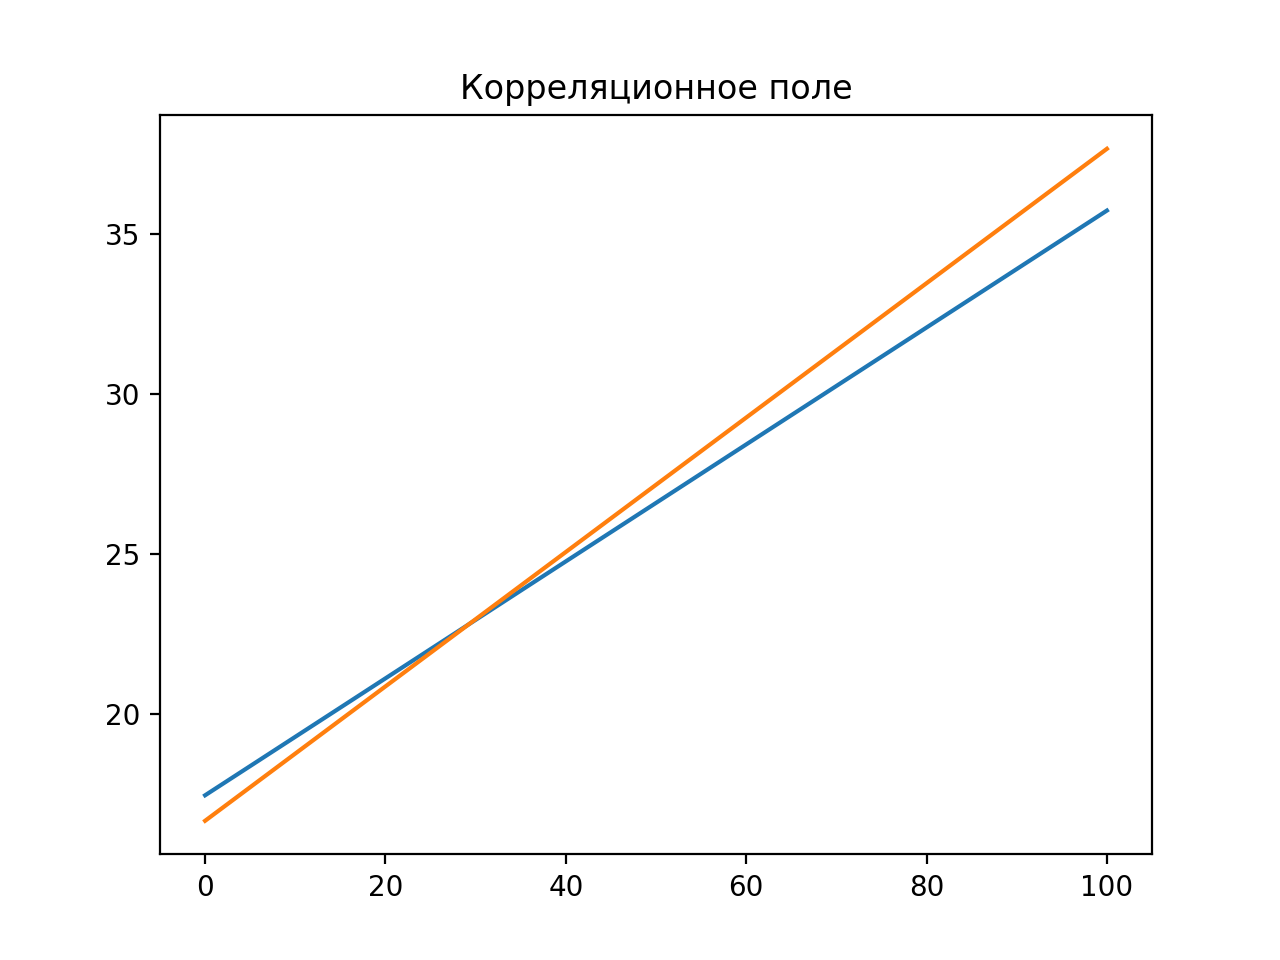
\includegraphics[width=0.9\textwidth]{src/gr31}

95\% доверительный интервал для коэффициентов регрессии.
Если уравнение имеет вид $\bar{y}_x = b_0 + b_1 x$, то $b_0 \in (-0.1754; 0.5409)$, а $b_1 \in (17.4456; 17.8154)$

Для оценки значимости выборочного коэффициента вычислим:
\begin{gather*}
    t_{watch} = r\sqrt{\frac{n-2}{1-r^2}} = 31.2775\\
    t_{crit} = 1.98\\
    t_{watch} > t_{crit}\\
\end{gather*}

Нулевую гипотезу отвергаем.
Коэффициент корреляции значимо отличается от нуля.